\documentclass[10pt]{article}

\usepackage{fullpage}
\usepackage{setspace}
\usepackage{parskip}
\usepackage{titlesec}
\usepackage{xcolor}
\usepackage{lineno}





\PassOptionsToPackage{hyphens}{url}
\usepackage[colorlinks = true,
            linkcolor = blue,
            urlcolor  = blue,
            citecolor = blue,
            anchorcolor = blue]{hyperref}
\usepackage{etoolbox}
\makeatletter
\patchcmd\@combinedblfloats{\box\@outputbox}{\unvbox\@outputbox}{}{%
  \errmessage{\noexpand\@combinedblfloats could not be patched}%
}%
\makeatother


\usepackage[round]{natbib}
\let\cite\citep




\renewenvironment{abstract}
  {{\bfseries\noindent{\abstractname}\par\nobreak}\footnotesize}
  {\bigskip}

\renewenvironment{quote}
  {\begin{tabular}{|p{13cm}}}
  {\end{tabular}}

\titlespacing{\section}{0pt}{*3}{*1}
\titlespacing{\subsection}{0pt}{*2}{*0.5}
\titlespacing{\subsubsection}{0pt}{*1.5}{0pt}


\usepackage{authblk}


\usepackage{graphicx}
\usepackage[space]{grffile}
\usepackage{latexsym}
\usepackage{textcomp}
\usepackage{longtable}
\usepackage{tabulary}
\usepackage{booktabs,array,multirow}
\usepackage{amsfonts,amsmath,amssymb}
\providecommand\citet{\cite}
\providecommand\citep{\cite}
\providecommand\citealt{\cite}
% You can conditionalize code for latexml or normal latex using this.
\newif\iflatexml\latexmlfalse
\providecommand{\tightlist}{\setlength{\itemsep}{0pt}\setlength{\parskip}{0pt}}%

\AtBeginDocument{\DeclareGraphicsExtensions{.pdf,.PDF,.eps,.EPS,.png,.PNG,.tif,.TIF,.jpg,.JPG,.jpeg,.JPEG}}

\usepackage[utf8]{inputenc}
\usepackage[english]{babel}








\begin{document}

\title{Project Overview}



\author{Garth Terlizzi, Parakh Jaggi}%
\affil{Estimated time worked on project:  65 hours each}%


\vspace{-1em}



  \date{\today}


\begingroup
\let\center\flushleft
\let\endcenter\endflushleft
\maketitle
\endgroup








\begin{quote}
\end{quote}

The Nutrition Trakr is a personal calorie and exercise tracker with Java
FX and Apache Derby implementation. After a quick registration and
survey, consisting of the user's height, weight, and dimensions the user
is free to start tracking calories with our database of categories and
foods. If the user eats a food that currently isn't in the database,
then he or she will have the option to add the food and the number of
calories that food has to the database. The user can also do the same
with exercises. The user can select an exercise that he or she has
completed, or they can add a new exercise for all users to see. The
users can also see their monthly progress with a colorful bar chart.

Although the Fitness Trakr seems like a single person app, the users can
actually compete with each other. Using our leaderboard, the users can
compare their Trakr scores and try to one up each other to get the
coveted first place. If you do not want to compete with other users, you
can still get a sense of accomplishment with our ribbon system. A great
Trakr score will give the user a Gold ribbon, an average score a Silver
ribbon, and a bad score a Bronze ribbon.

\begin{quote}
\end{quote}

The user will be able to register and the user account remains after the termination of the program. The user will be able to input what foods he has eaten for the day, and the calories associated with the food are added to their tracker.
The user will be able to input what foods he has eaten for the day, and the exercise associated with the food are added to their tracker.
The user will be able to view his Fitness Score, a calculation based off the information in his tracker.
The user should be able to view his BMI/ BFA.
The user should be able to see the graphs based on information from the trackers, regardless if there is a lack of information from the tracker.
The user will be able to view his Fitness Score compared to everyone else in the database, leaderboard style. 
The user should be able to view his goals and edit his goals.


\textbf{Usability:}

The program must have a working login/sign up page and a dashboard with
buttons leading to working pages.

The dashboard should be simple, with buttons leading to the actions.

The graphics should be monochromatic, not flashy.

The program should be well documented

\textbf{Reliability:}

The program should always open on start-up.

Input Errors should be validated.

Errors should result in a message box, then close the program.

\textbf{Performance:}

The program should have a relatively fast response time for database
retrieval.

The program should not use any threads or event that causes multiple
processes to run.

\textbf{Supportability:}

The program should be compatible on Windows and IOS devices.

\textbf{Business Rules:}

The user needs to have an account in order to access the dashboard.

The user should not create an account if their email is already tied to
another account.

The user should be able to use outside utilities (scale, tape measurer,
height-market) to know their BFA attributes.

The user should know how many calories they ate/burned from outside
sources if the information is not contained within the database.

\textbf{Vision Statement}

To provide an opportunity for health-conscious people to set their goals
and then track their lifestyle habits quantitatively and view their
progress over time.

\textbf{Junit Testing Analysis}

The Junit tests covers mostly database alteration, as our application is
a database-driven project. There are test cases resolving the inserts of
food, users, and tracker entries. We also test bad loads in SQL
statements (such as searching for a user that does not exist). Other
notable tests are a test that verifies that categories display all
values in a list, in the proper order, and a test that verifies a
leaderboard is initialized. However, with testing databases, we run the
risk of adding unnecessary data to the tables, eventually reducing the
access time of our SQL queries. To counteract that, we have created
delete functions that remove our test-case variables from our schema at
the end of each test. We also test the user class to verify that a male
user and female user output the correct body fat measurements and body
mass index. Because most of our functions are infused with the graphics,
it is hard to test anything other than database calls and functions.

\textbf{Use Cases:}\selectlanguage{english}
\begin{longtable}[]{@{}ll@{}}
\toprule
\begin{minipage}[t]{0.47\columnwidth}\raggedright\strut
Use Case ID:\strut
\end{minipage} & \begin{minipage}[t]{0.47\columnwidth}\raggedright\strut
UC Add Goal\strut
\end{minipage}\tabularnewline
\begin{minipage}[t]{0.47\columnwidth}\raggedright\strut
Scope:\strut
\end{minipage} & \begin{minipage}[t]{0.47\columnwidth}\raggedright\strut
Data Input and Collection\strut
\end{minipage}\tabularnewline
\begin{minipage}[t]{0.47\columnwidth}\raggedright\strut
Level:\strut
\end{minipage} & \begin{minipage}[t]{0.47\columnwidth}\raggedright\strut
User goal\strut
\end{minipage}\tabularnewline
\begin{minipage}[t]{0.47\columnwidth}\raggedright\strut
Stake Holders and Interests:\strut
\end{minipage} & \begin{minipage}[t]{0.47\columnwidth}\raggedright\strut
User- Person entering data for Fitness Trakr\strut
\end{minipage}\tabularnewline
\begin{minipage}[t]{0.47\columnwidth}\raggedright\strut
Description:\strut
\end{minipage} & \begin{minipage}[t]{0.47\columnwidth}\raggedright\strut
The user logs on, views their goals, and adds a new goal.\strut
\end{minipage}\tabularnewline
\begin{minipage}[t]{0.47\columnwidth}\raggedright\strut
Preconditions:\strut
\end{minipage} & \begin{minipage}[t]{0.47\columnwidth}\raggedright\strut
The user has an account registered within the database.\strut
\end{minipage}\tabularnewline
\begin{minipage}[t]{0.47\columnwidth}\raggedright\strut
Post conditions:\strut
\end{minipage} & \begin{minipage}[t]{0.47\columnwidth}\raggedright\strut
Data entry is saved, and the goal is stored in the database\strut
\end{minipage}\tabularnewline
\begin{minipage}[t]{0.48\columnwidth}\raggedright\strut
Main Success Scenario:\strut
\end{minipage} & \begin{minipage}[t]{0.48\columnwidth}\raggedright\strut
The user enters his username and password. The user is directed to the
dashboard. The user selects ``View Goals'' The user types a goal in the
text field The user submits the goal The goal appears on the goal
List\strut
\end{minipage}\tabularnewline
\begin{minipage}[t]{0.48\columnwidth}\raggedright\strut
Extensions:\strut
\end{minipage} & \begin{minipage}[t]{0.48\columnwidth}\raggedright\strut
1.* The input is entered wrong, and the program re-allows for proper
entry. 6.1 The user has more than 5 goals, in which case not all goals
are shown. 6.2 The user deletes a goal from the drop down list of goals.
6.2.1. The user accidentally deletes a goal, and which case he uses the
undo button.\strut
\end{minipage}\tabularnewline
\bottomrule
\end{longtable}\selectlanguage{english}
\begin{longtable}[]{@{}ll@{}}
\toprule
\begin{minipage}[t]{0.47\columnwidth}\raggedright\strut
Use Case ID:\strut
\end{minipage} & \begin{minipage}[t]{0.47\columnwidth}\raggedright\strut
UC Add Goal\strut
\end{minipage}\tabularnewline
\begin{minipage}[t]{0.47\columnwidth}\raggedright\strut
Scope:\strut
\end{minipage} & \begin{minipage}[t]{0.47\columnwidth}\raggedright\strut
Data Input and Collection\strut
\end{minipage}\tabularnewline
\begin{minipage}[t]{0.47\columnwidth}\raggedright\strut
Level:\strut
\end{minipage} & \begin{minipage}[t]{0.47\columnwidth}\raggedright\strut
User goal\strut
\end{minipage}\tabularnewline
\begin{minipage}[t]{0.47\columnwidth}\raggedright\strut
Stake Holders and Interests:\strut
\end{minipage} & \begin{minipage}[t]{0.47\columnwidth}\raggedright\strut
User- Person entering data for Fitness Trakr\strut
\end{minipage}\tabularnewline
\begin{minipage}[t]{0.47\columnwidth}\raggedright\strut
Description:\strut
\end{minipage} & \begin{minipage}[t]{0.47\columnwidth}\raggedright\strut
The user logs on, views their goals, and adds a new goal.\strut
\end{minipage}\tabularnewline
\begin{minipage}[t]{0.47\columnwidth}\raggedright\strut
Preconditions:\strut
\end{minipage} & \begin{minipage}[t]{0.47\columnwidth}\raggedright\strut
The user has an account registered within the database.\strut
\end{minipage}\tabularnewline
\begin{minipage}[t]{0.47\columnwidth}\raggedright\strut
Post conditions:\strut
\end{minipage} & \begin{minipage}[t]{0.47\columnwidth}\raggedright\strut
Data entry is saved, and the goal is stored in the database\strut
\end{minipage}\tabularnewline
\begin{minipage}[t]{0.48\columnwidth}\raggedright\strut
Main Success Scenario:\strut
\end{minipage} & \begin{minipage}[t]{0.48\columnwidth}\raggedright\strut
The user enters his username and password. The user is directed to the
dashboard. The user selects ``View Goals'' The user types a goal in the
text field The user submits the goal The goal appears on the goal
List\strut
\end{minipage}\tabularnewline
\begin{minipage}[t]{0.48\columnwidth}\raggedright\strut
Extensions:\strut
\end{minipage} & \begin{minipage}[t]{0.48\columnwidth}\raggedright\strut
1.* The input is entered wrong, and the program re-allows for proper
entry. 6.1 The user has more than 5 goals, in which case not all goals
are shown. 6.2 The user deletes a goal from the drop down list of goals.
6.2.1. The user accidentally deletes a goal, and which case he uses the
undo button.\strut
\end{minipage}\tabularnewline
\bottomrule
\end{longtable}\selectlanguage{english}
\begin{longtable}[]{@{}ll@{}}
\toprule
\begin{minipage}[t]{0.47\columnwidth}\raggedright\strut
Use Case ID:\strut
\end{minipage} & \begin{minipage}[t]{0.47\columnwidth}\raggedright\strut
UC Add Goal\strut
\end{minipage}\tabularnewline
\begin{minipage}[t]{0.47\columnwidth}\raggedright\strut
Scope:\strut
\end{minipage} & \begin{minipage}[t]{0.47\columnwidth}\raggedright\strut
Data Input and Collection\strut
\end{minipage}\tabularnewline
\begin{minipage}[t]{0.47\columnwidth}\raggedright\strut
Level:\strut
\end{minipage} & \begin{minipage}[t]{0.47\columnwidth}\raggedright\strut
User goal\strut
\end{minipage}\tabularnewline
\begin{minipage}[t]{0.47\columnwidth}\raggedright\strut
Stake Holders and Interests:\strut
\end{minipage} & \begin{minipage}[t]{0.47\columnwidth}\raggedright\strut
User- Person entering data for Fitness Trakr\strut
\end{minipage}\tabularnewline
\begin{minipage}[t]{0.47\columnwidth}\raggedright\strut
Description:\strut
\end{minipage} & \begin{minipage}[t]{0.47\columnwidth}\raggedright\strut
The user logs on, views their goals, and adds a new goal.\strut
\end{minipage}\tabularnewline
\begin{minipage}[t]{0.47\columnwidth}\raggedright\strut
Preconditions:\strut
\end{minipage} & \begin{minipage}[t]{0.47\columnwidth}\raggedright\strut
The user has an account registered within the database.\strut
\end{minipage}\tabularnewline
\begin{minipage}[t]{0.47\columnwidth}\raggedright\strut
Post conditions:\strut
\end{minipage} & \begin{minipage}[t]{0.47\columnwidth}\raggedright\strut
Data entry is saved, and the goal is stored in the database\strut
\end{minipage}\tabularnewline
\begin{minipage}[t]{0.48\columnwidth}\raggedright\strut
Main Success Scenario:\strut
\end{minipage} & \begin{minipage}[t]{0.48\columnwidth}\raggedright\strut
The user enters his username and password. The user is directed to the
dashboard. The user selects ``View Goals'' The user types a goal in the
text field The user submits the goal The goal appears on the goal
List\strut
\end{minipage}\tabularnewline
\begin{minipage}[t]{0.48\columnwidth}\raggedright\strut
Extensions:\strut
\end{minipage} & \begin{minipage}[t]{0.48\columnwidth}\raggedright\strut
1.* The input is entered wrong, and the program re-allows for proper
entry. 6.1 The user has more than 5 goals, in which case not all goals
are shown. 6.2 The user deletes a goal from the drop down list of goals.
6.2.1. The user accidentally deletes a goal, and which case he uses the
undo button.\strut
\end{minipage}\tabularnewline
\bottomrule
\end{longtable}\selectlanguage{english}
\begin{longtable}[]{@{}ll@{}}
\toprule
\begin{minipage}[t]{0.47\columnwidth}\raggedright\strut
Use Case ID:\strut
\end{minipage} & \begin{minipage}[t]{0.47\columnwidth}\raggedright\strut
UC Add Goal\strut
\end{minipage}\tabularnewline
\begin{minipage}[t]{0.47\columnwidth}\raggedright\strut
Scope:\strut
\end{minipage} & \begin{minipage}[t]{0.47\columnwidth}\raggedright\strut
Data Input and Collection\strut
\end{minipage}\tabularnewline
\begin{minipage}[t]{0.47\columnwidth}\raggedright\strut
Level:\strut
\end{minipage} & \begin{minipage}[t]{0.47\columnwidth}\raggedright\strut
User goal\strut
\end{minipage}\tabularnewline
\begin{minipage}[t]{0.47\columnwidth}\raggedright\strut
Stake Holders and Interests:\strut
\end{minipage} & \begin{minipage}[t]{0.47\columnwidth}\raggedright\strut
User- Person entering data for Fitness Trakr\strut
\end{minipage}\tabularnewline
\begin{minipage}[t]{0.47\columnwidth}\raggedright\strut
Description:\strut
\end{minipage} & \begin{minipage}[t]{0.47\columnwidth}\raggedright\strut
The user logs on, views their goals, and adds a new goal.\strut
\end{minipage}\tabularnewline
\begin{minipage}[t]{0.47\columnwidth}\raggedright\strut
Preconditions:\strut
\end{minipage} & \begin{minipage}[t]{0.47\columnwidth}\raggedright\strut
The user has an account registered within the database.\strut
\end{minipage}\tabularnewline
\begin{minipage}[t]{0.47\columnwidth}\raggedright\strut
Post conditions:\strut
\end{minipage} & \begin{minipage}[t]{0.47\columnwidth}\raggedright\strut
Data entry is saved, and the goal is stored in the database\strut
\end{minipage}\tabularnewline
\begin{minipage}[t]{0.48\columnwidth}\raggedright\strut
Main Success Scenario:\strut
\end{minipage} & \begin{minipage}[t]{0.48\columnwidth}\raggedright\strut
The user enters his username and password. The user is directed to the
dashboard. The user selects ``View Goals'' The user types a goal in the
text field The user submits the goal The goal appears on the goal
List\strut
\end{minipage}\tabularnewline
\begin{minipage}[t]{0.48\columnwidth}\raggedright\strut
Extensions:\strut
\end{minipage} & \begin{minipage}[t]{0.48\columnwidth}\raggedright\strut
1.* The input is entered wrong, and the program re-allows for proper
entry. 6.1 The user has more than 5 goals, in which case not all goals
are shown. 6.2 The user deletes a goal from the drop down list of goals.
6.2.1. The user accidentally deletes a goal, and which case he uses the
undo button.\strut
\end{minipage}\tabularnewline
\bottomrule
\end{longtable}


\textbf{System Operations}

\begin{enumerate}
\tightlist
\item
  Login()
\item
  Register()
\item
  LoadUser(Username)
\item
  AddCaloriesToFoodTracker(CategoryFood)
\item
  InputFitnessData(Height,Weight)
\item
  SetGoals()
\item
  calculateFitnessScore()
\item
  ViewData()
\end{enumerate}

\textbf{Operation Contracts}\selectlanguage{english}
\begin{longtable}[]{@{}ll@{}}
\toprule
\textbf{Name} & \textbf{ViewData()}\tabularnewline
\midrule
\endhead
\textbf{Responsibilities} & Shows the data in terms of graphs stemming
from the calories tracker\tabularnewline
\textbf{Cross-references} & UC Input Data/View Graphs\tabularnewline
\textbf{Output} & A calorie bar graph\tabularnewline
\textbf{Pre-condition} & A user has valid information in the calorie
data form\tabularnewline
\textbf{Post-condition} & A bar chart is created\tabularnewline
\bottomrule
\end{longtable}\selectlanguage{english}
\begin{longtable}[]{@{}ll@{}}
\toprule
\textbf{Name} & \textbf{ViewData()}\tabularnewline
\midrule
\endhead
\textbf{Responsibilities} & Shows the data in terms of graphs stemming
from the calories tracker\tabularnewline
\textbf{Cross-references} & UC Input Data/View Graphs\tabularnewline
\textbf{Output} & A calorie bar graph\tabularnewline
\textbf{Pre-condition} & A user has valid information in the calorie
data form\tabularnewline
\textbf{Post-condition} & A bar chart is created\tabularnewline
\bottomrule
\end{longtable}\selectlanguage{english}
\begin{longtable}[]{@{}ll@{}}
\toprule
\textbf{Name} & \textbf{ViewData()}\tabularnewline
\midrule
\endhead
\textbf{Responsibilities} & Shows the data in terms of graphs stemming
from the calories tracker\tabularnewline
\textbf{Cross-references} & UC Input Data/View Graphs\tabularnewline
\textbf{Output} & A calorie bar graph\tabularnewline
\textbf{Pre-condition} & A user has valid information in the calorie
data form\tabularnewline
\textbf{Post-condition} & A bar chart is created\tabularnewline
\bottomrule
\end{longtable}\selectlanguage{english}
\begin{longtable}[]{@{}ll@{}}
\toprule
\textbf{Name} & \textbf{ViewData()}\tabularnewline
\midrule
\endhead
\textbf{Responsibilities} & Shows the data in terms of graphs stemming
from the calories tracker\tabularnewline
\textbf{Cross-references} & UC Input Data/View Graphs\tabularnewline
\textbf{Output} & A calorie bar graph\tabularnewline
\textbf{Pre-condition} & A user has valid information in the calorie
data form\tabularnewline
\textbf{Post-condition} & A bar chart is created\tabularnewline
\bottomrule
\end{longtable}\selectlanguage{english}
\begin{longtable}[]{@{}ll@{}}
\toprule
\textbf{Name} & \textbf{ViewData()}\tabularnewline
\midrule
\endhead
\textbf{Responsibilities} & Shows the data in terms of graphs stemming
from the calories tracker\tabularnewline
\textbf{Cross-references} & UC Input Data/View Graphs\tabularnewline
\textbf{Output} & A calorie bar graph\tabularnewline
\textbf{Pre-condition} & A user has valid information in the calorie
data form\tabularnewline
\textbf{Post-condition} & A bar chart is created\tabularnewline
\bottomrule
\end{longtable}\selectlanguage{english}
\begin{longtable}[]{@{}ll@{}}
\toprule
\textbf{Name} & \textbf{ViewData()}\tabularnewline
\midrule
\endhead
\textbf{Responsibilities} & Shows the data in terms of graphs stemming
from the calories tracker\tabularnewline
\textbf{Cross-references} & UC Input Data/View Graphs\tabularnewline
\textbf{Output} & A calorie bar graph\tabularnewline
\textbf{Pre-condition} & A user has valid information in the calorie
data form\tabularnewline
\textbf{Post-condition} & A bar chart is created\tabularnewline
\bottomrule
\end{longtable}\selectlanguage{english}
\begin{longtable}[]{@{}ll@{}}
\toprule
\textbf{Name} & \textbf{ViewData()}\tabularnewline
\midrule
\endhead
\textbf{Responsibilities} & Shows the data in terms of graphs stemming
from the calories tracker\tabularnewline
\textbf{Cross-references} & UC Input Data/View Graphs\tabularnewline
\textbf{Output} & A calorie bar graph\tabularnewline
\textbf{Pre-condition} & A user has valid information in the calorie
data form\tabularnewline
\textbf{Post-condition} & A bar chart is created\tabularnewline
\bottomrule
\end{longtable}\selectlanguage{english}
\begin{longtable}[]{@{}ll@{}}
\toprule
\textbf{Name} & \textbf{ViewData()}\tabularnewline
\midrule
\endhead
\textbf{Responsibilities} & Shows the data in terms of graphs stemming
from the calories tracker\tabularnewline
\textbf{Cross-references} & UC Input Data/View Graphs\tabularnewline
\textbf{Output} & A calorie bar graph\tabularnewline
\textbf{Pre-condition} & A user has valid information in the calorie
data form\tabularnewline
\textbf{Post-condition} & A bar chart is created\tabularnewline
\bottomrule
\end{longtable}


\textbf{Justification of Grasps}

\textbf{Controller:} We used Controller to carryout user interactions
with the home screen of the app. For example, if the user choses to open
the add calories screen, then the dashboard controller will handle the
user interaction (mouse click) and give a call to the add calorie
controller which will handle all user input and add it to the database.

\textbf{Creator:} Throughout the project we had to use many temporary
arrays to retrieve data from the database. We made these arrays using
the creator grasp and the Abstract Factory design pattern. This really
refined our code and made the creation of new Arrays easier to
implement.

\textbf{High Cohesion:} Each screen that shows up in our app has a
unique controller class which only deals with the methods and on-screen
objects for that screen. This implementation uses high cohesion which
makes each function specific to its rule and makes it not have more
responsibility than it needs.

\textbf{Indirection} : To separate the database statements and the Java
FX code we created a class to indirectly connect the two. This allows
for cleaner code and reusability. The DatabaseGateway class inserts,
selects, removes objects from the database that is inputted by the user.
This means that the controller classes and the database code could be
reused if needed by another project.

\textbf{Information Expert:} To ensure that each system action is
delegated to a class we used Information Expert. This allowed us to
create a class for each controller, which delegated each screens
responsibility to a controller, so no class is doing two classes worth
of work.

\textbf{Low Coupling:} We integrated Low coupling by ensuring that each
User has no awareness to a Goal or Food. All the User has is a calorie
count which is linked to food and goals using the database as a
middleman.

\textbf{Polymorphism:} Polymorphism is used in the Female and Male
users. The equations for calculating Body Mass Index is different for
males and females. So, the Male User and FemaleUser is inherited from
the User super class. We also use it to delegate different database
functions base on functionality

\textbf{Pure Fabrication:} To ensure Low Coupling and High Cohesion we
had to create a controller and a Database gateway. These two made it so
each class is specific to its role and so classes will not know about
each other if they don't need to. We also used the DatbaseGateway as
fabricated classes to ensure access to the database.

\textbf{Do Not Talk To Strangers:} Users have no interaction with other
users, and Goals and Calories have no interaction with each other. This
ensures that no class is interacting with an unrelated class. The only
classes that have a relation with each other are the ones that need to.

\textbf{Design Patterns}

\textbf{Singleton:} To interact with the Database in our app, an
instance of the DatabaseGateway class must be created. Since
DatabaseGateway has the potential to modify the data in the database, we
are only allowing one instance of it at any time, using singleton. This
lowers the risk of unnecessary interaction between the Database and the
rest of the application. If a method requires an instance of the
DatabaseGateway the class will return the same instance over and over so
that there is never more than one instance.

\textbf{Abstract Factory:} When interacting with the database the
creation of temporary ArrayLists was necessary. When selecting Food,
Calories, or Goals, an ArrayList would have to be created to hold the
large amounts of data. In order to support reusability and code
arbitration we used a ListFactory to produce a List whenever a
controller needs one.

\textbf{Command:} To promote high cohesion we made a controller class to
handle each screen that is viewable by the user. Since each of these
controllers have to execute a command to display, the command pattern
was used. This allows us to use the controller.execute method on each
controller and assume that it will successfully open the page.

\textbf{Observer:} When updating a user's information many different
fields must be filled. If a field becomes changed, then the database
must be notified in order for the data to be saved. This is implemented
as an observer pattern. The observer pattern allows us to notify all
observers anytime a field is changed, which in return will update the
database.

\textbf{State:} We wanted to reward the user with a ribbon if their
FitnessScore is good. A user can get a Gold ribbon for a great score, a
Silver ribbon for a okay score, and a Bronze ribbon for a bad score. In
order to recognize the level at which the user is currently in we used
the State pattern. This allows the system to know how which ribbon the
user deserves at all times.

\textbf{Prototype} : The user has the ability to add, remove, and undo
goals. When undoing a goal, a copy of the goal must be created so that
the goal can be added back into the database. This happens through the
prototype pattern. The goal gets cloned using the cloneable interface
and gets sent to the database using an instance of the DatabaseGateway.

\textbf{Memento:} When the user deletes a goal, the goal must be saved
somewhere so that an undo will add the goal back to the goal list. These
deleted goals are saved using the Memento pattern. A deleted goal will
be saved into an arrayList created by the Factory, and then held until
the user requests the goal to be undoed.



\begin{figure}[p!]
	\begin{center}
		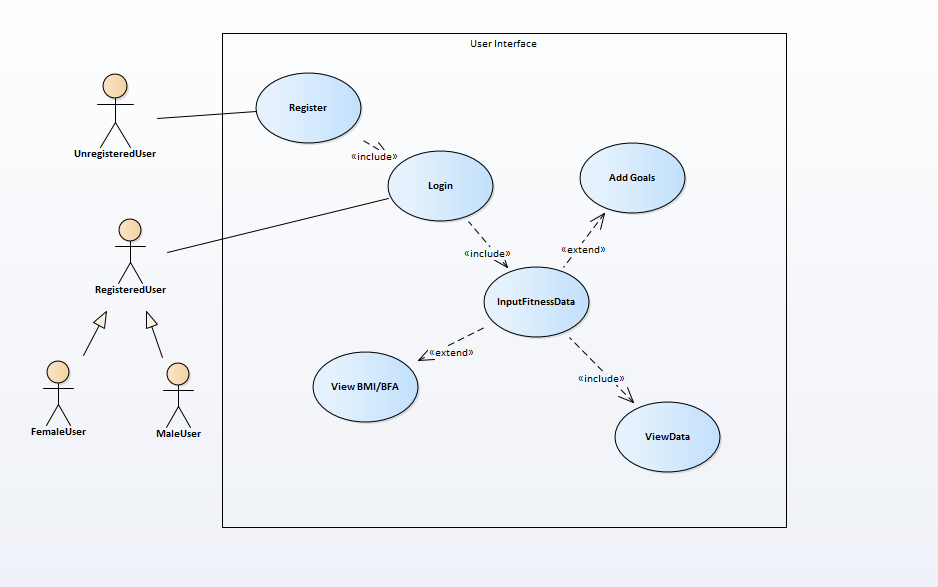
\includegraphics[width=\columnwidth]{UseCaseModel.jpg}
		\caption{{USE CASE MODEL
				{\label{div-915296}}%
		}}
	\end{center}
\end{figure}


\begin{figure}[p!]
	\begin{center}
		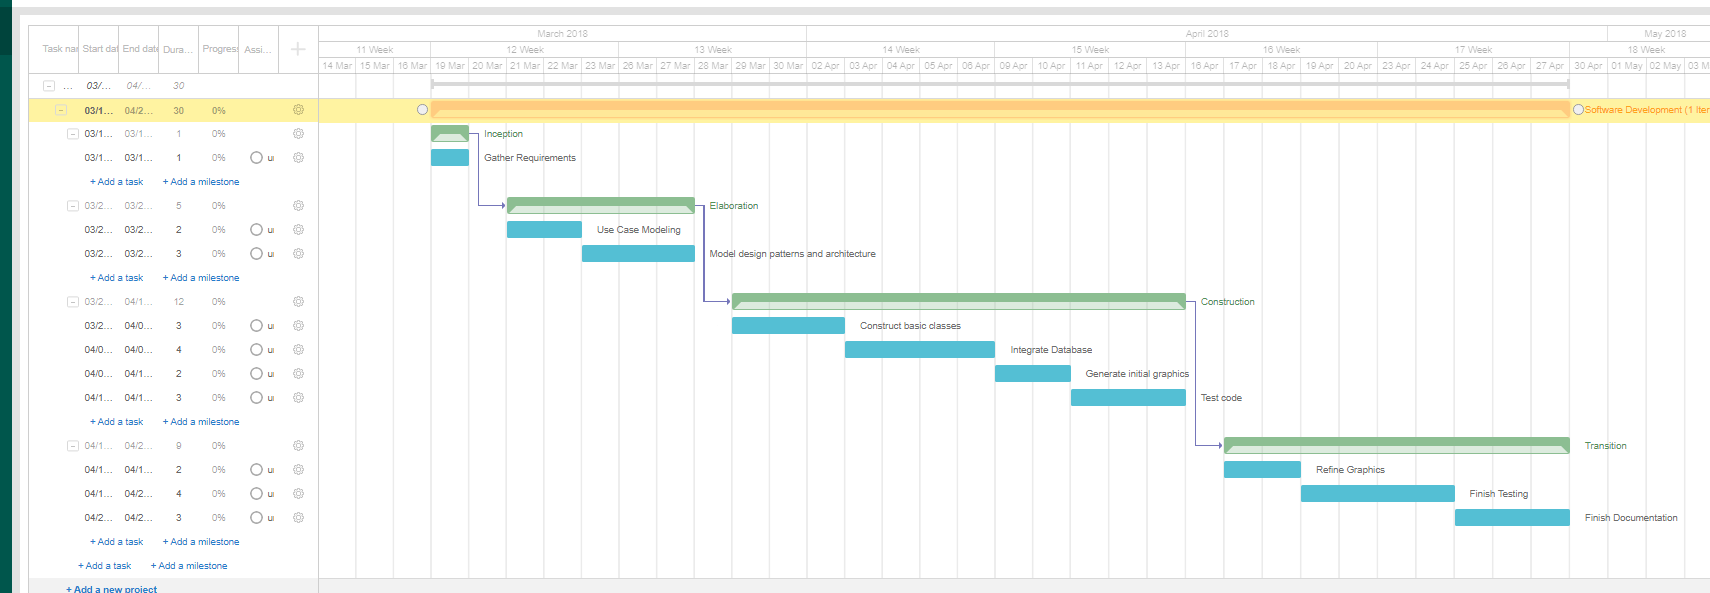
\includegraphics[width=\columnwidth]{Gannt1.png}
		\caption{{GANNT DIAGRAM
				{\label{div-327881}}%
		}}
	\end{center}
\end{figure}


\begin{figure}[p!]
	\begin{center}
		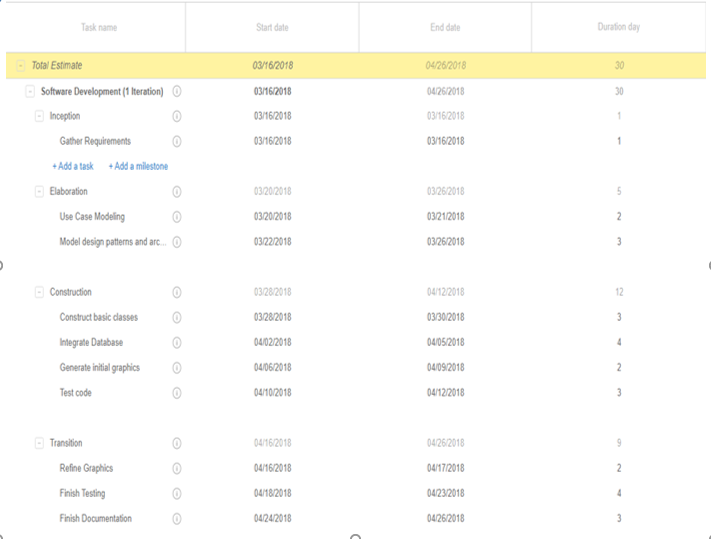
\includegraphics[width=\columnwidth]{GANNTCHART.png}
		\caption{{GANNT CHART
				{\label{div-381784}}%
		}}
	\end{center}
\end{figure}


\begin{figure}[p!]
	\begin{center}
		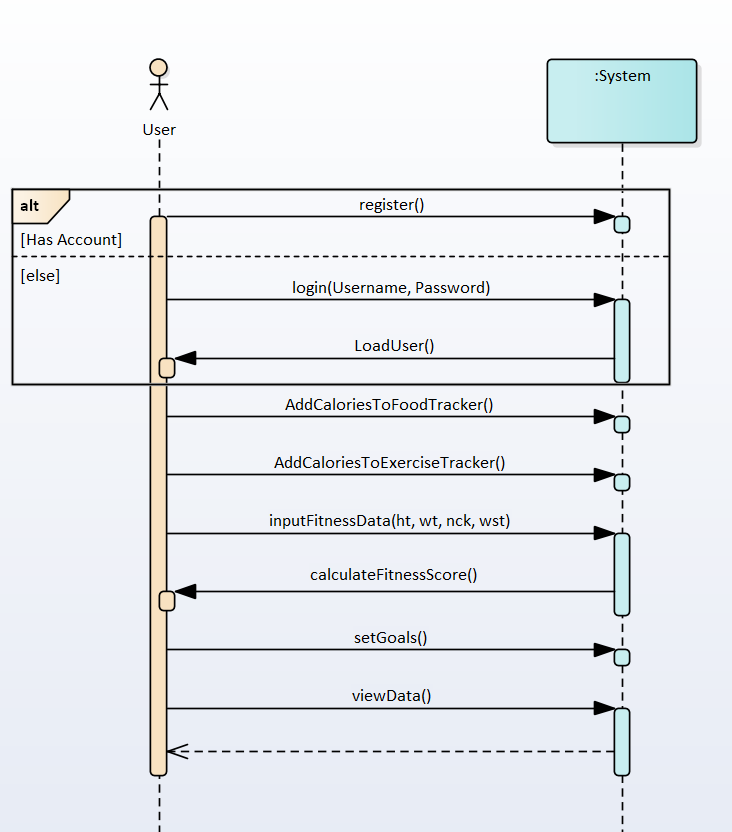
\includegraphics[width=\columnwidth]{SSD.png}
		\caption{{SYSTEM SEQUENCE DIAGRAM
				{\label{div-941985}}%
		}}
	\end{center}
\end{figure}



\begin{figure}[h!]
	\begin{center}
		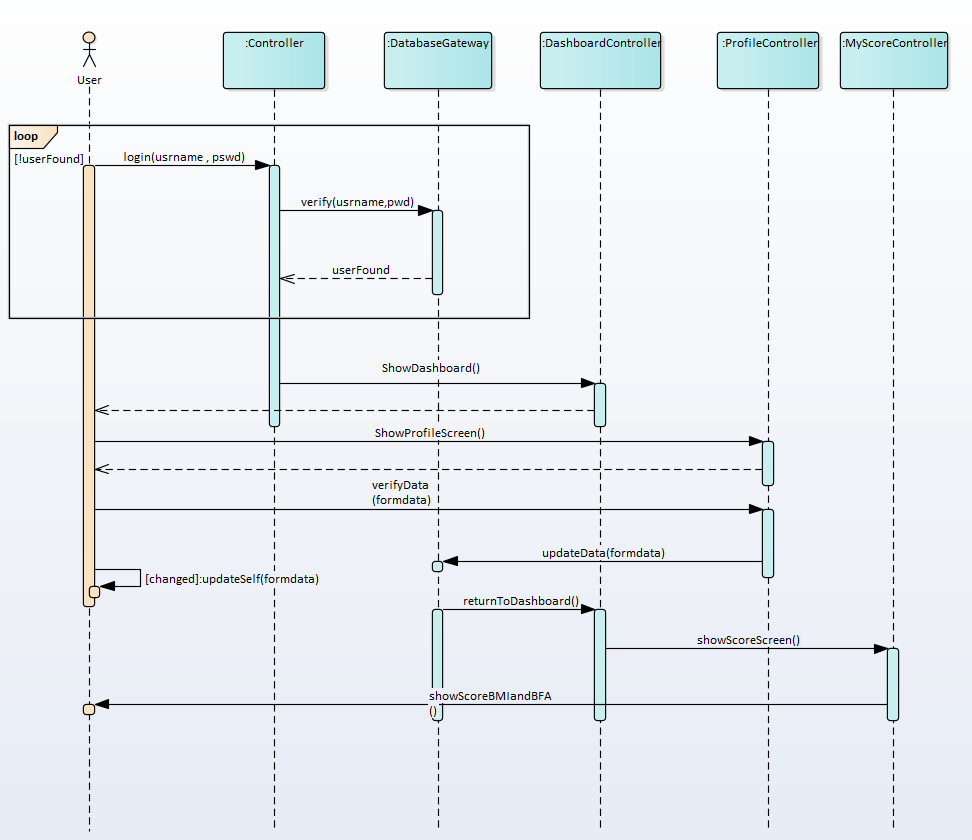
\includegraphics[width=\columnwidth]{UC1.png}
		\caption{{Sequence Diagram (UC View BFA,BMI, FitnessScore)
				{\label{div-391931}}%
		}}
	\end{center}
\end{figure}


\begin{figure}[h!]
	\begin{center}
		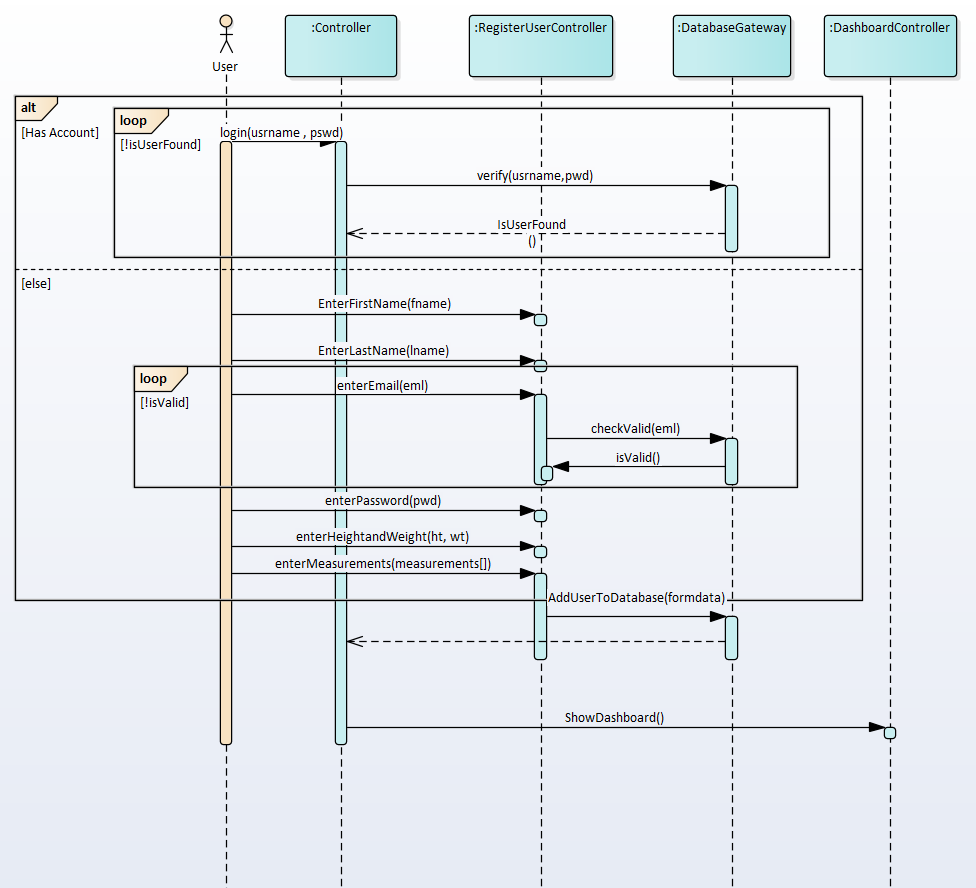
\includegraphics[width=\columnwidth]{UC2.png}
		\caption{{Sequence Diagram (UC View Dashboard)
				{\label{div-475015}}%
		}}
	\end{center}
\end{figure}


\begin{figure}[h!]
	\begin{center}
		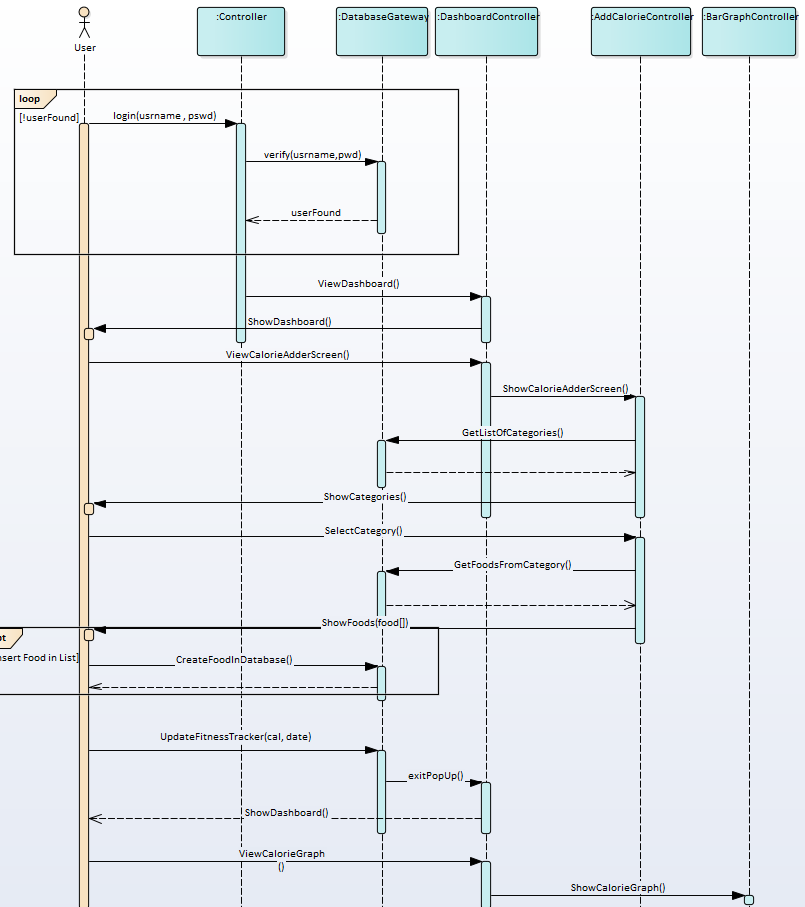
\includegraphics[width=\columnwidth]{UC3.png}
		\caption{{Sequence Diagram (UC Input Data/View Graphs)
				{\label{div-885174}}%
		}}
	\end{center}
\end{figure}


\begin{figure}[h!]
	\begin{center}
		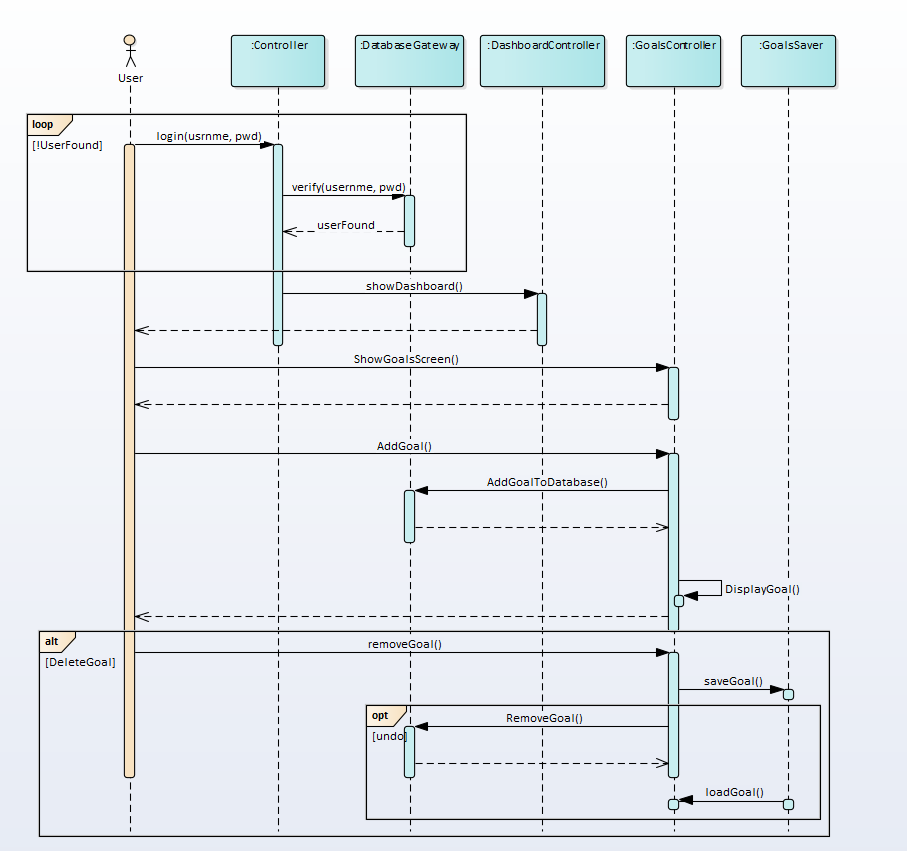
\includegraphics[width=\columnwidth]{UC4.png}
		\caption{{Sequence Diagram (Add Goal)
				{\label{div-291050}}%
		}}
	\end{center}
\end{figure}


\begin{figure}[h!]
	\begin{center}
		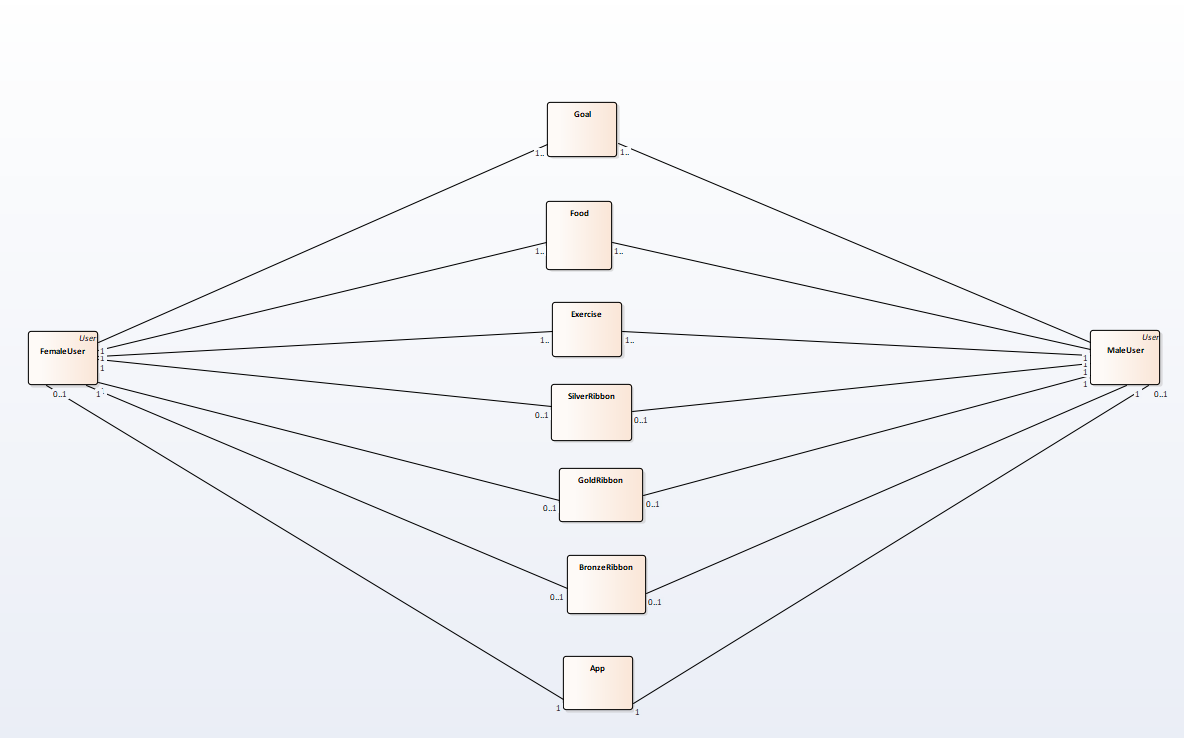
\includegraphics[width=\columnwidth]{Domain.png}
		\caption{{Domain Model
				{\label{div-291050}}%
		}}
	\end{center}
\end{figure}


\begin{figure}[h!]
	\begin{center}
		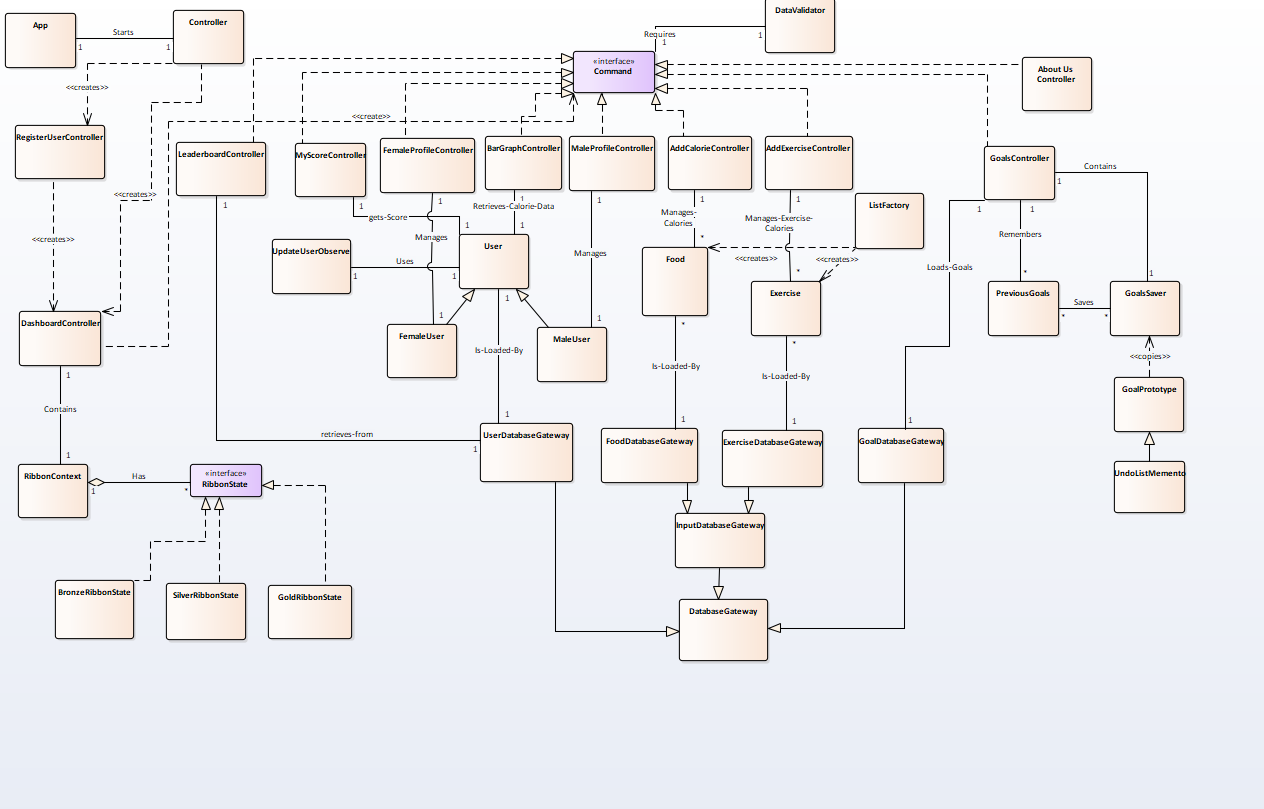
\includegraphics[width=\columnwidth]{DesignBasic.png}
		\caption{{Design Model (Basic)
				{\label{div-291050}}%
		}}
	\end{center}
\end{figure}


\begin{figure}[h!]
	\begin{center}
		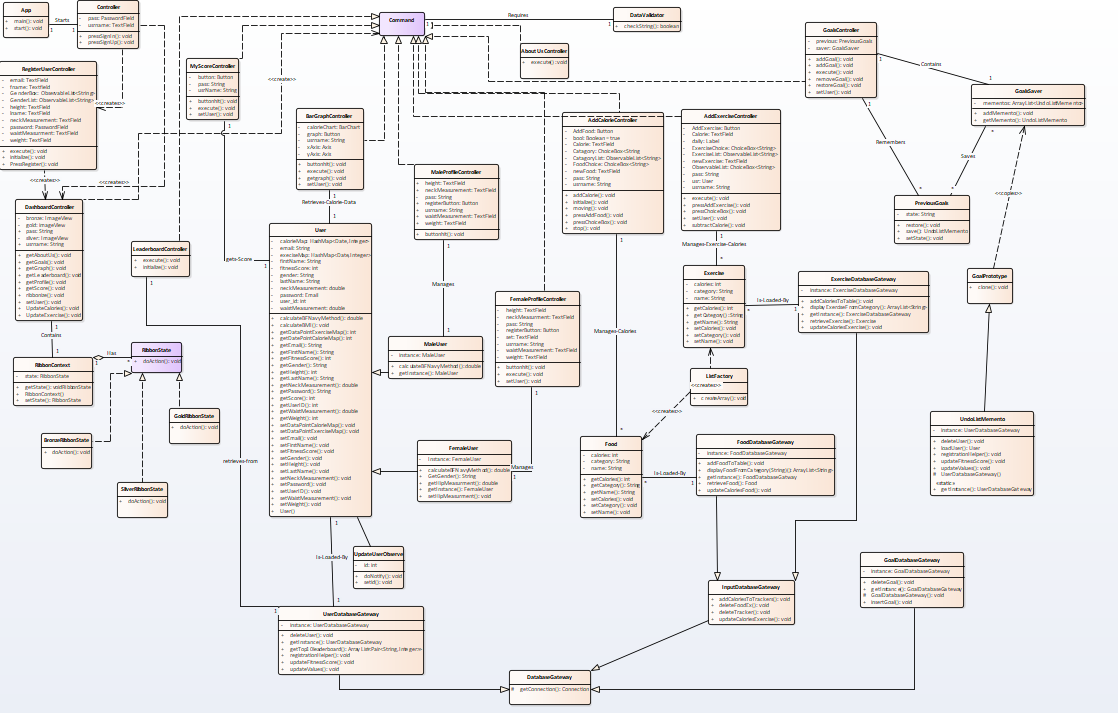
\includegraphics[width=\columnwidth]{DesignFull.png}
		\caption{{Design Model (FullyDressed)
				{\label{div-291050}}%
		}}
	\end{center}
\end{figure}
\selectlanguage{english}
\clearpage
\end{document}

